%%% Hlavní soubor. Zde se definují základní parametry a odkazuje se na ostatní části. %%%

%% Verze pro jednostranný tisk:
% Okraje: levý 40mm, pravý 25mm, horní a dolní 25mm
% (ale pozor, LaTeX si sám přidává 1in)
\documentclass[12pt,a4paper]{report}
\setlength\textwidth{145mm}
\setlength\textheight{247mm}
\setlength\oddsidemargin{15mm}
\setlength\evensidemargin{15mm}
\setlength\topmargin{0mm}
\setlength\headsep{0mm}
\setlength\headheight{0mm}
% \openright zařídí, aby následující text začínal na pravé straně knihy
\let\openright=\clearpage

%% Pokud tiskneme oboustranně:
% \documentclass[12pt,a4paper,twoside,openright]{report}
% \setlength\textwidth{145mm}
% \setlength\textheight{247mm}
% \setlength\oddsidemargin{15mm}
% \setlength\evensidemargin{0mm}
% \setlength\topmargin{0mm}
% \setlength\headsep{0mm}
% \setlength\headheight{0mm}
% \let\openright=\cleardoublepage

%% Pokud používáte csLaTeX (doporučeno):
%\usepackage{czech}
%% Pokud nikoliv:
\usepackage[slovak]{babel} % aby mi nepisalo Obrazek ;-)
%\usepackage[T1]{fontenc}

%% Použité kódování znaků: obvykle latin2, cp1250 nebo utf8:
\usepackage[utf8]{inputenc}

%% Ostatní balíčky
\usepackage{graphicx}
\usepackage{amsthm}
\usepackage{epstopdf}
\newtheorem{theorem}{Veta}
\newtheorem{define}{Definícia}	
\newtheorem{note}{Poznámka}
\newtheorem{example}{Príklad}
\newtheorem{consequence}{Dôsledok}


\usepackage{amsfonts} % matematika
%\usepackage{graphicx} % svg grafika % zbytocne???

\usepackage{graphicx}

% 5 kvoli velkemu Ocku pre casovu zlozitost
\usepackage{amsmath}
\usepackage{amssymb}
\usepackage{mathtools}

\newcommand{\BigO}[1]{\ensuremath{\operatorname{O}\bigl(#1\bigr)}}


% mnoziny
\newcommand{\N}{\mathbb{N}\,}
\newcommand{\Z}{\mathbb{Z}\,}
\newcommand{\Q}{\mathbb{Q}\,}
\newcommand{\R}{\mathbb{R}\,}
\newcommand{\Ri}{\mathbb{R}^{*}\,}


\usepackage{listings} % zdrojaky c++
\usepackage{color}
\usepackage{xcolor}

\lstset { %
belowcaptionskip=1\baselineskip,
breaklines=true,
showstringspaces=false,
basicstyle=\footnotesize\ttfamily,
keywordstyle=\bfseries\color{green!40!black},
commentstyle=\itshape\color{purple!40!black},
identifierstyle=\color{blue},
stringstyle=\color{orange},
backgroundcolor=\color{black!5},
tabsize=4
}


%\usepackage[linesnumbered,ruled,vlined]{algorithm2e}
\usepackage{algorithm}

\usepackage{algorithmic} % http://ftp.cvut.cz/tex-archive/macros/latex/contrib/algorithms/algorithms.pdf
\floatname{algorithm}{Algoritmus}
\renewcommand{\algorithmicrequire}{\textbf{Vstup:}}
\renewcommand{\algorithmicensure}{\textbf{Výstup:}}
\renewcommand{\algorithmiccomment}[1]{\{#1\}}


\usepackage[toc,page]{appendix}
\renewcommand{\appendixtocname}{Prílohy}
\renewcommand\appendixname{Príloha}
\renewcommand\appendixpagename{Prílohy}
  

%% Balíček hyperref, kterým jdou vyrábět klikací odkazy v PDF,
%% ale hlavně ho používáme k uložení metadat do PDF (včetně obsahu).
%% POZOR, nezapomeňte vyplnit jméno práce a autora.
\usepackage[unicode]{hyperref}   % Musí být za všemi ostatními balíčky
\hypersetup{pdftitle=Grid-Based Path Planning}
\hypersetup{pdfauthor=Tomáš Novella}

%%% Drobné úpravy stylu

% Tato makra přesvědčují mírně ošklivým trikem LaTeX, aby hlavičky kapitol
% sázel příčetněji a nevynechával nad nimi spoustu místa. Směle ignorujte.
\makeatletter
\def\@makechapterhead#1{
  {\parindent \z@ \raggedright \normalfont
   \Huge\bfseries \thechapter. #1
   \par\nobreak
   \vskip 20\p@
}}
\def\@makeschapterhead#1{
  {\parindent \z@ \raggedright \normalfont
   \Huge\bfseries #1
   \par\nobreak
   \vskip 20\p@
}}
\makeatother

% Toto makro definuje kapitolu, která není očíslovaná, ale je uvedena v obsahu.
\def\chapwithtoc#1{
\chapter*{#1}
\addcontentsline{toc}{chapter}{#1}
}

\begin{document}

% Trochu volnější nastavení dělení slov, než je default.
\lefthyphenmin=2
\righthyphenmin=2

%%% Titulní strana práce

\pagestyle{empty}
\begin{center}

\large

Univerzita Karlova v Praze

\medskip

Matematicko-fyzikální fakulta

\vfill

{\bf\Large BAKALÁRSKA PRÁCA}

\vfill

\centerline{\mbox{\includegraphics[width=60mm]{./img/logo.eps}}}

\vfill
\vspace{5mm}

{\LARGE Tomáš Novella}

\vspace{15mm}

% Název práce přesně podle zadání
{\LARGE\bfseries Grid-Based Path Planning}

\vfill

% Název katedry nebo ústavu, kde byla práce oficiálně zadána
% (dle Organizační struktury MFF UK)
Katedra teoretické informatiky a matematické logiky

\vfill

\begin{tabular}{rl}

Vedúci bakalárskej práce: & Mgr. Tomáš Balyo \\
\noalign{\vspace{2mm}}
Študijný program: & Informatika \\
\noalign{\vspace{2mm}}
Študijný obor: & Obecná informatika \\
\end{tabular}

\vfill

% Zde doplňte rok
Praha 2013

\end{center}

\newpage

%%% Následuje vevázaný list -- kopie podepsaného "Zadání bakalářské práce".
%%% Toto zadání NENÍ součástí elektronické verze práce, nescanovat.

%%% Na tomto místě mohou být napsána případná poděkování (vedoucímu práce,
%%% konzultantovi, tomu, kdo zapůjčil software, literaturu apod.)

\openright

\noindent
Poďakovanie.

\newpage

%%% Strana s čestným prohlášením k bakalářské práci

\vglue 0pt plus 1fill

\noindent
Prehlasujem, že som túto prácu vypracoval samostatne a výhradne
s~použitím citovaných prameňov, literatúry a ďalších
odborných zdrojov.


\medskip\noindent
Beriem na~vedomie, že sa na moju prácu vzťahujú práva
a povinnosti vyplývajúce zo zákona  č. 121/2000 Sb.,
autorského zákona a v~platnom znení, obzvlášť skutočnosť,
že Univerzita Karlova v Prahe má právo na~uzavretie licenčnej zmluvy o~použití tejto práce ako školského diela podľa
§60 odst. 1 autorského zákona.

\vspace{10mm}

\hbox{\hbox to 0.5\hsize{%
V ........ dne ............
\hss}\hbox to 0.5\hsize{%
Podpis autora
\hss}}

\vspace{20mm}
\newpage

%%% Povinná informační strana bakalářské práce

\vbox to 0.5\vsize{
\setlength\parindent{0mm}
\setlength\parskip{5mm}

Názov práce:
Grid-Based Path Planning
% přesně dle zadání

Autor:
Tomáš Novella

Katedra:  % Případně Ústav:
Katedra teoretické informatiky a matematické logiky
% dle Organizační struktury MFF UK

Vedúci bakalárskej práce:
Mgr. Tomáš Balyo, Katedra teoretické informatiky a
matematické logiky
% dle Organizační struktury MFF UK, případně plný název pracoviště mimo MFF UK

Abstrakt:
% abstrakt v rozsahu 80-200 slov; nejedná se však o opis zadání bakalářské práce

Kľúčové slová:
% 3 až 5 klíčových slov

\vss}\nobreak\vbox to 0.49\vsize{
\setlength\parindent{0mm}
\setlength\parskip{5mm}

Title:
Grid-Based Path Planning
% přesný překlad názvu práce v angličtině

Author:
Tomáš Novella

Department:
Department of Theoretical Computer Science and Mathematical Logic
% dle Organizační struktury MFF UK v angličtině

Supervisor:
Mgr. Tomáš Balyo, Department of Theoretical Computer Science and
Mathematical Logic
% dle Organizační struktury MFF UK, případně plný název pracoviště
% mimo MFF UK v angličtině

Abstract:
% abstrakt v rozsahu 80-200 slov v angličtině; nejedná se však o překlad
% zadání bakalářské práce

Keywords:
% 3 až 5 klíčových slov v angličtině

\vss}

\newpage

%%% Strana s automaticky generovaným obsahem bakalářské práce. U matematických
%%% prací je přípustné, aby seznam tabulek a zkratek, existují-li, byl umístěn
%%% na začátku práce, místo na jejím konci.

\openright
\pagestyle{plain}
\setcounter{page}{5}
\tableofcontents


%%% Jednotlivé kapitoly práce jsou pro přehlednost uloženy v samostatných souborech
\chapter*{Úvod}
\addcontentsline{toc}{chapter}{Úvod}

Slávna Eulerova úloha siedmych mostov v Kaliningrade \cite{euler41} sa považuje za prvú prácu, 
ktorá zaviedla teóriu grafov.
Úlohou je prejsť po týchto siedmych mostoch tak, aby sme po každom prešli práve raz.


\begin{figure}[h]
\centering
\includegraphics[height=7.5cm]{./img/Konigsberg_bridges.png}
\caption{Sedem mostov v Kaliningrade, \url{http://en.wikipedia.org/wiki/Seven_Bridges_of_K\%C3\%B6nigsberg}}
\label{fig:konigsberg_bridges}
\end{figure}

 
Od tej doby sa využitie teórie grafov značne
rozšírilo a v dnešnej dobe patrí medzi významné
a rozpracované teórie. V modernej dobe je jedným z jej 
naj\-dô\-le\-ži\-tej\-ších 
problémov hľadanie najkratšej cesty. Najčastejšie sa s~nimi stretávame pri plánovaní trasy v~GPS navigácii.
Medzi najvýznamnešie práce považujeme práce od Dijkstru \cite{dijkstra59} a Floyd-Warshalla \cite{floyd62}.

So~začiatkom fenoménu počítačových hier 
a umelej inteligencie sa do povedomia dostal špeciálny typ grafu --
mriežkový graf, využívaný ako herná mapa.
V~hrách často trebalo nájsť cestu pre počítačom
ovládanú postavičku z miesta A do miesta B.
Nakoľko je väčšina hier komerčná, algoritmy
využívané v~hrách boli a~sú taktiež komerčné.
Dôsledkom toho nie sú verejne publikované a~porovnané rôzne prístupy a~algoritmy
na~vyhľadávanie (ideálne najkratších) ciest v~mriežkových mapách. A~keď už aj sú, tak práce používajú rôzne mapy
na~bechmarking a~teda neexistuje žiadna globálna porovnávacia štúdia týchto prístupov.

Súťaž {\sl Grid-Based Path Planning Competition}
 \cite{sturtevantgppc} sa snaží tento problém vyriešiť tým, že porovnáva rôzne algoritmy na~veľkej množine máp
použitých v~známych počítačových hrách a~vyhodnocuje ich úspešnosť v~rámci viacerých kategórií.

Cieľom tejto práce je spraviť prehľad doterajších prístupov k~tomuto problému, zistiť ich vlastnosti a~prispieť vlastným algoritmom do sútaže s~niekoľkými vylepšeniami k~doterajším prístupom hľadania najkratšej cesty na~mriežkových grafoch.

V prvej kapitole si zavedieme kľúčové termíny a~popíšeme problém formálne. Na~konci kapitoly spomenieme súťaž, ktorej sa daný algoritmus zúčastnil.
Druhá kapitola je zameraná na~vytvorenie prehľadu kľúčových algoritmov použivaných na~riešenie problému.
V~ďalšej kapitole navrhneme vlastné riešenie založené na~poznatkoch popísaných v~druhej kapitole s~pridaním vlastných vylepšení.
A v poslednej kapitole toto riešenie porovnáme s dosavadnými.

Práca obsahuje dve prílohy: stručnú užívateľskú a programátorskú do\-ku\-men\-tá\-ciu programu \emph{T-maps}, ktorý slúži na grafické zobrazenie mriežkového grafu.


\part{Analýza problému}
\chapter{Zadanie problému a cieľové požiadavky}

\section{Úvodné definície a značenia}
Na začiatok si zaveďme niektoré dôležité pojmy z teórie grafov.
Úlohu so všetkými jej špecifikami si ozrejmíme v nasledujúcich podkapitolách.
\begin{define}
{\sl Graf G} je usporiadaná dvojica (V, E), kde V označuje množinu vrcholov(vertices) a $E \subseteq V \times V $ označuje množinu hrán (edges). Značíme G = (V, E).
\end{define}


\begin{note}
Hrana je jednoznačne určená dvojicou vrcholov.
\end{note}


\begin{define}
{\sl Ohodnotený graf (G, w)} je graf s~spolu s~reálnou funkciou (tzv. ohodnotením)
$w: E(G) \to \R$, kde $w$ je funkcia, ktorá každej hrane priradí
reálne číslo takzvanú \emph{dĺžku}, alebo \emph{hodnotu} hrany.
\end{define}

Ukážka obecného ohodnoteného grafu je na obrázku \ref{fig:ohodnoteny_graf}.

\begin{figure}[h]
\centering
\includegraphics[height=5.5cm]{./img/graf.eps}
\caption{Ohodnotený graf}
\label{fig:ohodnoteny_graf}
\end{figure}

Pri hľadaní najkratšej cesty v grafe pracujeme s pojmamy, ako 
sú \emph{cesta} a \emph{najkratšia cesta}.

\begin{define}
{\sl Cesta P z vrcholu $v_0$ do vrcholu $v_n$ v grafe G } je postupnosť $P = (v_{0},e_{1},v_{1},\dots, e_{n}, v_{n})$,
pre ktorú platí $e_{i} = \{v_{i-i},v_{i}\}$ a taktiež
$v_{i} \ne v_{j}$ pre každé $i \ne j$.
\end{define}

Všimnime si, že na ceste nenavštívime žiaden vrchol dvakrát a teda cesta neobsahuje kružnice.


\begin{define}
{\sl Dĺžka cesty P z vrcholu $v_0$ do vrcholu $v_n$ v ohodnotenom grafe (G, w) } je súčet dĺžok hrán, ktoré sa na~ceste nachádzajú.
\end{define}

Samozrejme, medzi dvoma vrcholmi môže existovať viacero ciest.

\begin{define}
{\sl Najkratšia cesta P z vrcholu $v_0$ do vrcholu $v_n$
v~ohodnotenom grafe (G, w)} 
je cesta z~vrcholu $v_0$ do vrcholu $v_n$ s najmenšou dĺžkou. 
\end{define}


\section{Mriežkový graf}

Keď sme si už zaviedli kľúčové pojmy, prejdime k samotnému
zadaniu úlohy.
Ako sme už spomínali, problém budeme riešit na tzv. mriežkových grafoch. Čo je mriežkový graf a v čom sa od obecného grafu odlišuje?

V hernej praxi predstavuje mriežkový graf mapu hracej plochy, s ktorou sa stretávame v najrôznejších hrách, ako je Warcraft, Startcraft, Dragon Age \cite{sturtevant2012benchmarks}
a~podobne.

Ide o špeciálny a dosť obmedzený typ grafu. Vizuálne si ho môžme predstaviť ako konečný graf v ktorom sú vrcholy rozostúpené v tvare mriežky a hrana
je stále medzi dvojicami susedných vrcholov vo všetkých ôsmych smeroch. Dĺžka vodorovnej alebo zvislej hrany je $1$ a dĺžka šikmej hrany je $\sqrt{2}$.

\begin{note}
Mriežkový graf patrí medzi {\sl riedke} grafy,
pretože má veľmi malý počet hrán (lineárny od počtu vrcholov).
\end{note}


\begin{figure}[h]
\centering
\includegraphics[height=3.5cm]{./img/mriezkovy_graf2x2.eps}
\caption{Mriežkový graf 2x2}
\label{fig:mriezkovy_graf2x2}
\end{figure}


\begin{figure}[h]
\centering
\includegraphics[height=5.5cm]{./img/mriezkovy_graf.eps}
\caption{Mriežkový graf bez označenia vrcholov a dĺžok hrán}
\label{fig:mriezkovy_graf}
\end{figure}


Zadefinujme si teraz mriežkový graf formálne.

\begin{define}
{\sl Mriežkový graf rozmerov $m \times n$} je ohodnotený graf s~ohodnotením $w$ s m*n vrcholmi očíslovanými od $v_{1,1}$ až po $v_{m,n}$ 
s~priamymi hranami $j$ v~tvare $\{v_{a,b}, v_{a,b+1}\}, \{v_{a,b}, v_{a+1,b}\}$, kde $w(j) = 1$ 
a šikmými hranami $ s $ v~tvare 
$\{v_{a,b}, v_{a+1,b+1}\}$, $\{v_{a,b}, v_{a-1,b+1}\}$, kde $ w(s) = \sqrt{2}$.
\end{define}

\begin{note}
	Mriežkový graf sa dá reprezentovať ako matica $m \times n$ nad telesom $\Z_2$, kde jednotky predstavujú vrcholy. 
\end{note}
\begin{example}
Mriežkový graf rozmerov $2 \times 2$ s vyznačenými dĺžkami
hrán vidíme na obrázku~\ref{fig:mriezkovy_graf2x2}.
Príklad mriežkového grafu $4 \times 7$ je na obrázku~\ref{fig:mriezkovy_graf}.
Príklad jeho maticovej reprezentácie je na obrázku~\ref{fig:maticova_reprezentacia}.

\end{example}


\begin{figure}[h]


\[
G =
  \begin{bmatrix}
    1 & 0 & 1 & 1 & 1 & 1 & 0\\
	1 & 1 & 1 & 0 & 1 & 0 & 1\\
	1 & 1 & 1 & 1 & 0 & 0 & 1\\
	1 & 1 & 0 & 1 & 1 & 1 & 1\\
  \end{bmatrix}
\]

\caption{Maticová reprezentácia mriežkového grafu}
\label{fig:maticova_reprezentacia}
\end{figure}




\section{GPPC: Grid-Based Path Planning Competition}
Algoritmus navrhnutý a naprogramovaný v tejto práci bol zaradený do súťaže \textbf{GPPC}, ktorá sa koná približne raz ročne.

\subsection{Špecifiká súťaže, limity}

Mriežkové grafy budú mať rozmery maximálne $2048 \times 2048$.
Súťaž bude rozdelená do dvoch fáz --- fázy predspracovania grafu (pre-processing)
a fázy testovania. Na predspracovanie grafu bude vyhradený čas
maximálne 30 minút a program si svoje dáta uloží na disk do súboru o veľkosti maximálne 50MB.
Potom vo fáze testovania budé dostávať požiadavky na nájdenie najkratšej cesty. Úlohou je naimplementovať interface zobrazený na obrázku \ref{fig:interface}. ASK?? obrazku???a ked nie obrazk, tak ake cislovanie tomu dat? cislovat znovu od jednicky?

\begin{figure}
\begin{lstlisting}[language=C++]
struct xyLoc 
{
    int x;
    int y;
};

void PreprocessMap(std::vector<bool> &bits, int width, int height, const char *filename);
                   
void *PrepareForSearch(std::vector<bool> &bits, int width, int height,const char *filename);

bool GetPath(void *data, xyLoc s, xyLoc g, std::vector &path);
\end{lstlisting}
\caption{Interface, ktorý treba naimplementovať}
\label{fig:interface}
\end{figure}
Funkcia \emph{PreprocessMap} má za úlohu predspracovať
mriežkový graf a vytvoriť si pomocné dátové štruktúry podľa predpísaných limitov. Jej prvým argumentom 
je samotný mriežkový graf predaný ako zlinearizovaná matica, ktorú bolo vidieť na obrázku~\ref{fig:maticova_reprezentacia}. Ďalšími argumentami sú rozmery grafu,
keďže z jednorozmernej reprezentácie nie sú odvoditeľné. Posledným argumentom je názov súboru, do ktorého sa pomocné dátové štruktúry uložia.

Funkcia \emph{PrepareForSearch} slúži na načítanie dát z vytvoreného súboru. Argumenty má rovnaké, ako predošlá funkcia. Štvrtý argument
dodáva názov súboru, z ktorého sa pomocné dáta načítajú. Funkcia po načítaní dát skonštruuje dátové štruktúry a vráti na nich smerník.

Tento smerník prevezme v prvom argumente funkcia \emph{GetPath}, ktorá slúži na nájdenie najkratšej cesty. Jej ďalšími argumentami
sú súradnice počiatočného a koncového bodu, pre ktoré sa bude hľadať cesta a posleným argumentom je referencia na vektor, do ktorého sa samotná cesta uloží. Funkcia vracia hodnotu typu boolean na základe toho, či už vypočítala istý úsek a chce vrátiť cestu. Zíde sa napríklad, keď treba vrátiť čo najrýchlejšie aspoň prvých $k$ krokov cesty (viď.~Kritériá, sekcia~\ref{kriteria}).



\subsection{Kritériá súťaže, hodnotenie programov}
Na algoritmus môžeme klásť rôzne požiadavky, ktoré si častokrát navzájom protirečia, preto programy posudzujeme poďla viacerých kritérií.
\label{kriteria}
\begin{itemize}
\item Celkový čas na~nájdenie cesty.
\item Čas na nájdenie prvých 20 tich krokov.
\item Dĺžka cesty (zohľadnená suboptimalita).
\item Maximálny čas vrátenia hociktorej časti cesty.
\end{itemize}

Testovací počítač má 12 GB RAM pamäti a dva 2.4 Ghz Intel Xeon E5620
procesory.
\chapter{Prehľad algoritmov}
Na hľadanie najkratších ciest v grafe poznáme mnoho algoritmov, ktoré rozdeľujeme do týchto troch \cite{mares07} skupín: 


\begin{itemize}
\item Point To Point Shortest Path(P2PSP) - hľadajú najkratšiu cestu medzi dvoma zadanými bodmi.
\item Single Source Shortest Path(SSSP) - pre daný vrchol {\sl v} hľadajú najkratšiu cestu do všetkých vrcholov grafu.
\item All Pairs Shortest Path (APSP)- skúmajú najkratšiu cestu medzi všetkými dvojicami vrcholov.
\end{itemize}

Tieto problémy sú na obecných grafoch NP-ťažké.
Napriek tomu na mriežkových grafoch (kde sú vzdialenosti medzi vrcholmi vždy kladné) existujú algoritmy v polynomiálnom čase.

V práci sa budeme ďalej zaoberať riešením prvého problému (Point to Point Shortest Path). 

V tejto kapitole popíšeme algoritmy, ktoré sú použiteľné na grafoch s nezápornými dĺžkami hrán. 


\section{Kritériá efektivity algoritmu}
Na porovnanie efektivity algoritmou slúži v teoretickej informatike odhad asymptotickej složitosti \cite{asymptotic65}.
Tento odhad je veľmi užitočný v teoretickej informatike a veľmi často algoritmus s lepšou zložitosťou je v praxi rýchlejší.
Nie je to ale pravidlom a teda potrebujeme zaviesť ďalšie kritériá, ktoré presnejšie popíšu a porovnajú správanie algoritmov v praxi.
Kritéria, podľa ktorých budeme porovnávať efektivitu algoritmov sú teda nasledovné:
\begin{itemize}
	\item Asymptotická zložitosť.
	\item Počet navštívených vrcholov.
	\item Reálny čas behu algoritmu.
\end{itemize}



\section{Dijkstrov algoritmus}
Medzi základné algoritmy typu SSSP patrí Dijkstrov algoritmus \cite{dijkstra59} popísaný už v roku 1959. 
Miernu modifikáciu pôvodného algoritmu môžeme vidieť na Algoritme \ref{alg:dijkstra}). 
Patrí medzi relaxačné algoritmy~a zbehne korektne na grafoch
s nezápornými hranami.

Pri hľadaní cesty z vrcholu $s$ do vrcholu $t$ prechádzame postupne vrcholy s neklesajúcou vzdialenosťou od $s$, až dokým sa nedostaneme k cieľovému vrcholu $t$.

Vrchol môže byť v jednom z troch stavov: NENAVŠTÍVENÝ, OTVORENÝ a ZATVORENÝ.
Nenavštívený bude vrchol, do ktorého sme ešte ani nezačali hľadať najkratšiu cestu. Vrchol je otvorený, keď sme našli najkratšiu cestu 
k~nejakému jeho susedovi a vrchol je uzavretý, pokiaľ sme už k~nemu našli najkratšiu cestu.
V algoritme budeme používať minimovú haldu, ktorá vracia vrcholy s najmenšou vzdialenosťou.
Vrchol sa po vložení do haldy automaticky otvára.

Na začiatku sú všetky vrcholy v~stave NENAVŠTÍVENÝ a~vložíme do~haldy počiatočný vrchol.
Postupne z~haldy vyberáme vrcholy a~po~vybratí ich uzavrieme. 
Po~vybraní otvoreného vrcholu prejdeme všetkých jeho neuzavretých susedov a pokiaľ sme k nim našli cestu kratšiu, ako bola dosiaľ nájdená, tak ich~vložíme do~haldy.


\begin{algorithm}
\caption{Dijkstra: zisti vzdialenosť najkratšej cesty z vrcholu $s$ do všetkých dostupných vrcholov}
\label{alg:dijkstra}
\begin{algorithmic}[1] % number one = line numbering is on
\REQUIRE graf $G$
\ENSURE dĺžková funkcia $d$ obsahujúca najkratšie cesty  z vrcholu $s$ do vrcholov grafu


\STATE $ d(*) \leftarrow \infty $
\STATE $ stav(*) \leftarrow$ NENAVŠTÍVENÝ

\STATE // pridám počiatok
\STATE $d(s) \leftarrow 0$
\STATE $stav(s) \leftarrow $ OTVORENÝ
\STATE Heap $H$
\STATE $Insert(H, s)$

\WHILE {$H$  not empty}
	
	\STATE // vyberieme v --- najbližší otvorený vrchol
	\STATE $v \leftarrow ExtractMin(H)$
	
	\WHILE {$stav(v) \neq $ OTVORENÝ}
		\STATE $v \leftarrow ExtractMin(H)$
	\ENDWHILE
	\STATE $stav(v) \leftarrow$ UZAVRETÝ
	\STATE // zrelaxujeme vrchol $v$
	\FORALL {$e$, $e = (v, u)$}
		\IF {$d(u) > d(v) + l(v, u)$}
			\STATE $Insert(H, v)$
			\STATE $stav(u) \leftarrow$ OTVORENÝ
			\STATE $d(u) \leftarrow d(v) + l(v, u)$
			
		\ENDIF
	\ENDFOR
\ENDWHILE

\end{algorithmic}
\end{algorithm}

\begin{theorem}
V dijkstrovom algoritme uzatvárame každý dosiahnuteľný vrchol práve raz.
\end{theorem}
\begin{proof}
Napríklad \cite{mares07}.
\end{proof}

\subsection{Zložitosť}
Každý vrchol vložíme do haldy maximálne $deg(v)$-krát 
(v najhoršom prípade postupne vyberáme z haldy jeho susedov a cez každého nasledujúceho suseda vedie kratšia cesta k vrcholu $v$ -- teda ho stále pridáme znovu).
Počet všetkých vložení bude teda rádovo $\BigO{\sum_{v}{deg(v)}} = \BigO{m}$.
Zo štruktúry môžme vybrať maximálne toľko prvkov, koľko sme tam vložili a~teda aj volania $ExtractMin$ trvajú $\BigO{m}$.

Algoritmus zbehne v čase $\BigO{m T_i + m T_e}$, kde $T_i$ odpovedá času na vloženie prvku a $T_d$ odpovedá času na vybranie najmenšieho prvku.

To znamená, že zložitosť algoritmu závisí od zložitosti operácií $Insert$ a $ExtractMin$. Na riedke grafy je obecne v praxi najvýhodnejšie použiť 
binárnu haldu, ktorej obe operácie trvajú $\BigO{\log{n} } $ a celkový čas je 
 $\BigO{m\log{n}}$
Prehľad štruktúr aj so zložitosťami operácií $Insert$ a $ExtractMin$ sa nachádza napr. v \cite{mares07}.

\subsection{Halda na mriežkovom grafe}
Nakoľko mriežkový graf je veľmi špeciálny typ grafu,
vieme niektoré jeho vlastnosti využiť na~to, aby sme vytvorili štruktúru, ktorá zvládne obe operácie v~konštantnom čase. 


Na konštrukciu tejto štruktúry (viď. \cite{gs97}) budeme potrebovať nasledujúcu vetu.

\begin{theorem}
\label{dinic-observation}
Pokiaľ sme v Dijkstrovom algoritme uzavreli vrchol $u$ so vzdialenosťou $d(u)$ a~najkratšia hrana v~grafe má dĺžku $\epsilon$, tak môžme taktiež 
uzavrieť všetky vrcholy $v$ so~vzdialenosťami $d(v) \in (d, d + \epsilon)$.
\end{theorem}
\begin{proof}
Do haldy vieme pridávať len vrcholy so~vzdialenosťami aspoň $d + \epsilon$ (kratšia hrana tam už nie je), 
ale~tie už cestu k~vrcholom so~vzdialenosťami
$d_v \in (d, d + \epsilon)$ skrátiť nemôžu.
\end{proof}


\begin{consequence}
Keď uzavrieme vrchol so vzdialenosťou $d_u$, môžme uzavrieť aj vrcholy so vzdialenosťami menšími, ako $d_u + \epsilon$
pričom poradie je nezávislé od skutočnej vzdialenosti vrcholov.
\end{consequence}

\begin{example}
\label{ex:range}
Dĺžka $\epsilon$ najkratšej hrany v mriežkovom grafe je 1. Je to dĺžka akejkoľvek vodorovnej, alebo zvislej hrany.
Keď teda uzavrieme vrchol so vzdialenosťou $d(u)$, môžme uzavrieť aj vrcholy so vzdialenosťami menšími, ako je $d(u) + 1$ a to v ľubovoľnom poradí.
\end{example}

Tieto skutočnosti vieme výborne využiť pri konštrukcii štruktúry
zvanej {\sl priehradková halda}. Tá, využijúc vyššie uvedenú vetu, uzatvára a pridáva vrcholy bez porušenia akejkoľvek konzistencie behu algoritmu.

\subsection{Popis haldy}
Najprv popíšeme fungovanie haldy a graficky znázorníme jej 
operácie. Neskôr dokážeme, že keď túto haldu použijeme v Dijkstrovom algoritme, tak nám bude vracať korektné výsledky.

Majme haldu s tromi priehradkami (nazvime ju $BucketHeap$), pričom rozsah jednej priehradky je ostro menší ako 1.
Prvá priehradka uchováva prvky s rozsahom vzdialeností
$ [b, b+1) $, druhá $ [b+1, b+2) $ a tretia $ [b+2, b+1+\sqrt{2}) $
pre danú bázu $ b $. Pre jednoduchšiu implementáciu $b \in \N$. Operácia $push((dist, data))$ vloží do haldy prvok so vzdialenosťou $dist$ 
s pomocnými dátami $data$. Operácia $pop()$ vracia ľubovoľný element z prvej priehradky. 
Pre jednoduchšiu implementáciu budeme mať na začiatku smerník na prvý prvok prvej priehradky a po vyhodení najmenšieho prvku tento smerník jednoducho inkrementujeme, kým to bude možné. Keď už v prvej priehradke nezostane žiaden prvok a zavoláme operáciu $pop()$, vykoná sa nasledujúca operácia: druhú priehradku presunieme na miesto prvej, tretiu na miesto druhej a prvú dáme namiesto tretej.

Ilustrujme si to na obrázkových príkladoch. Príklad troj--priehradkovej haldy vidíme na obrázku \ref{fig:priehradky}.
Halda uchováva premennú $ baza $ definujúcu bázu, od ktorej sa rozsahy priehradok odvíjajú. Okrem
nej, uchováva tri smerníky na tri po sebe idúce priehradky a smerník na vrchol haldy, zvaný $ top $.



\begin{figure}[h]
\centering
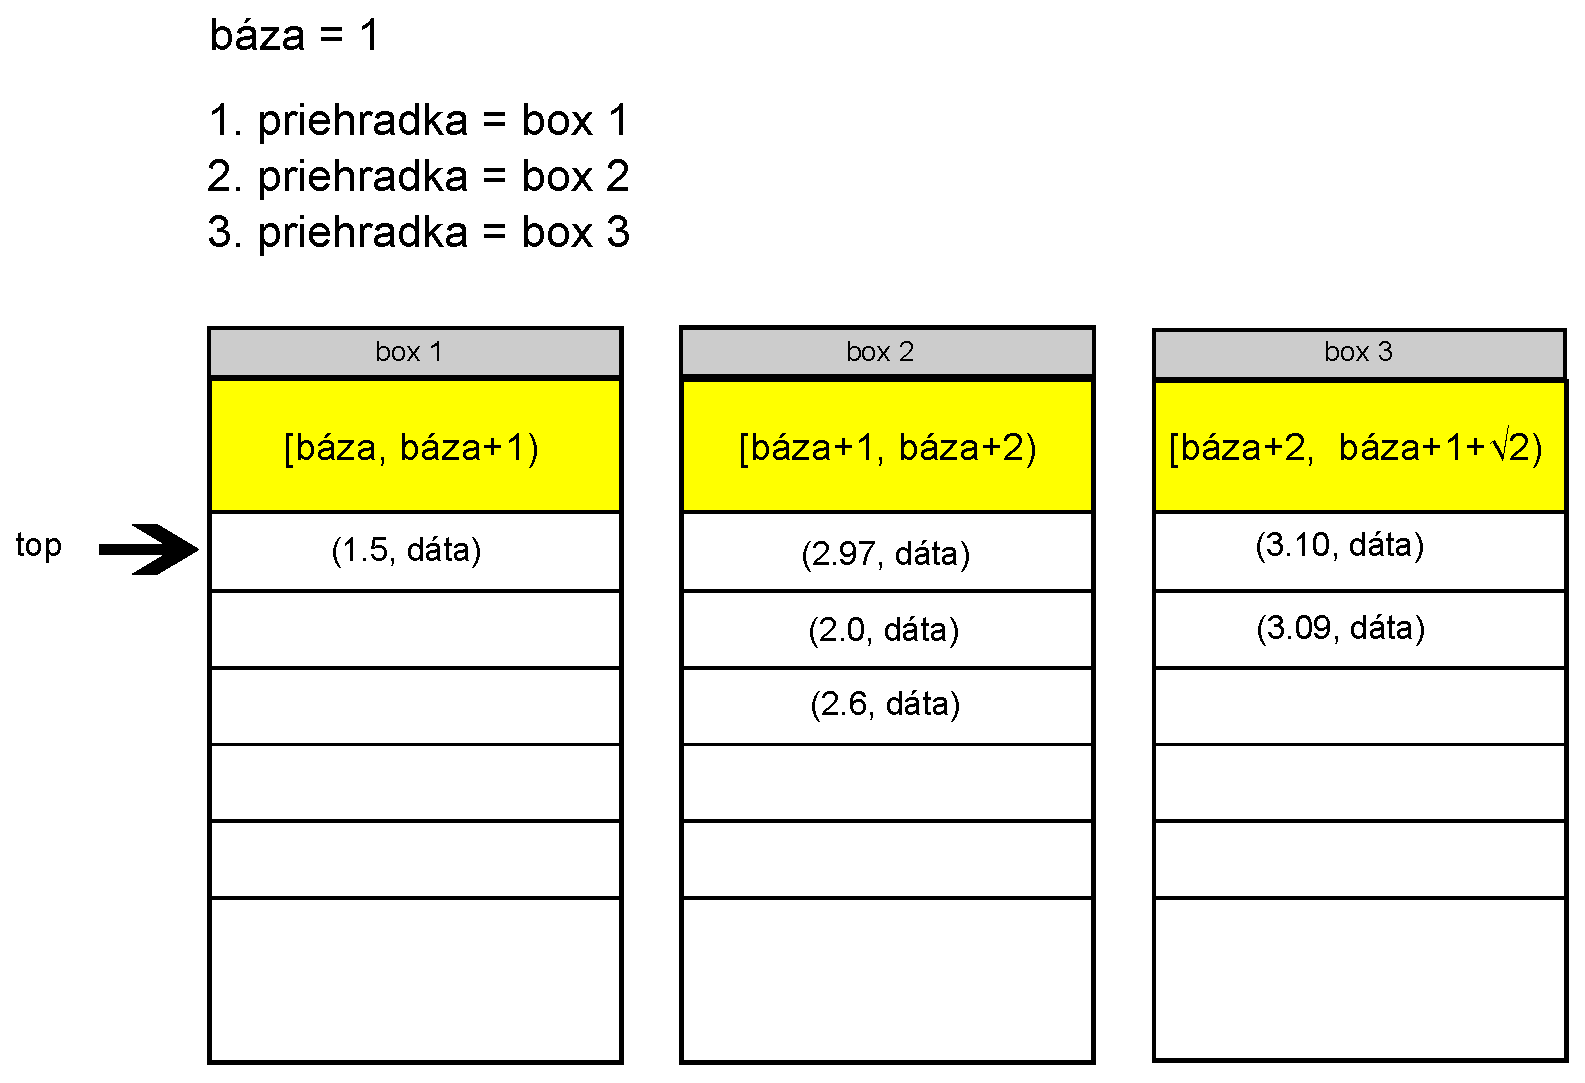
\includegraphics[width=\textwidth]{./img/priehradky_naplnene_default.eps}
\caption{Priehradková štruktúra s niekoľkými prvkami.}
\label{fig:priehradky}
\end{figure}

Pridanie dvoch prvkov je znázornené na obrázku \ref{fig:priehradky_i}. Priehradka, do ktorej má byť prvok s danou vzdialenosťou vložený sa vypočíta podľa vzorca:\\
 $ \lfloor vzdialenostPrvku - baza +1 \rfloor $.


\begin{figure}[h]
\centering
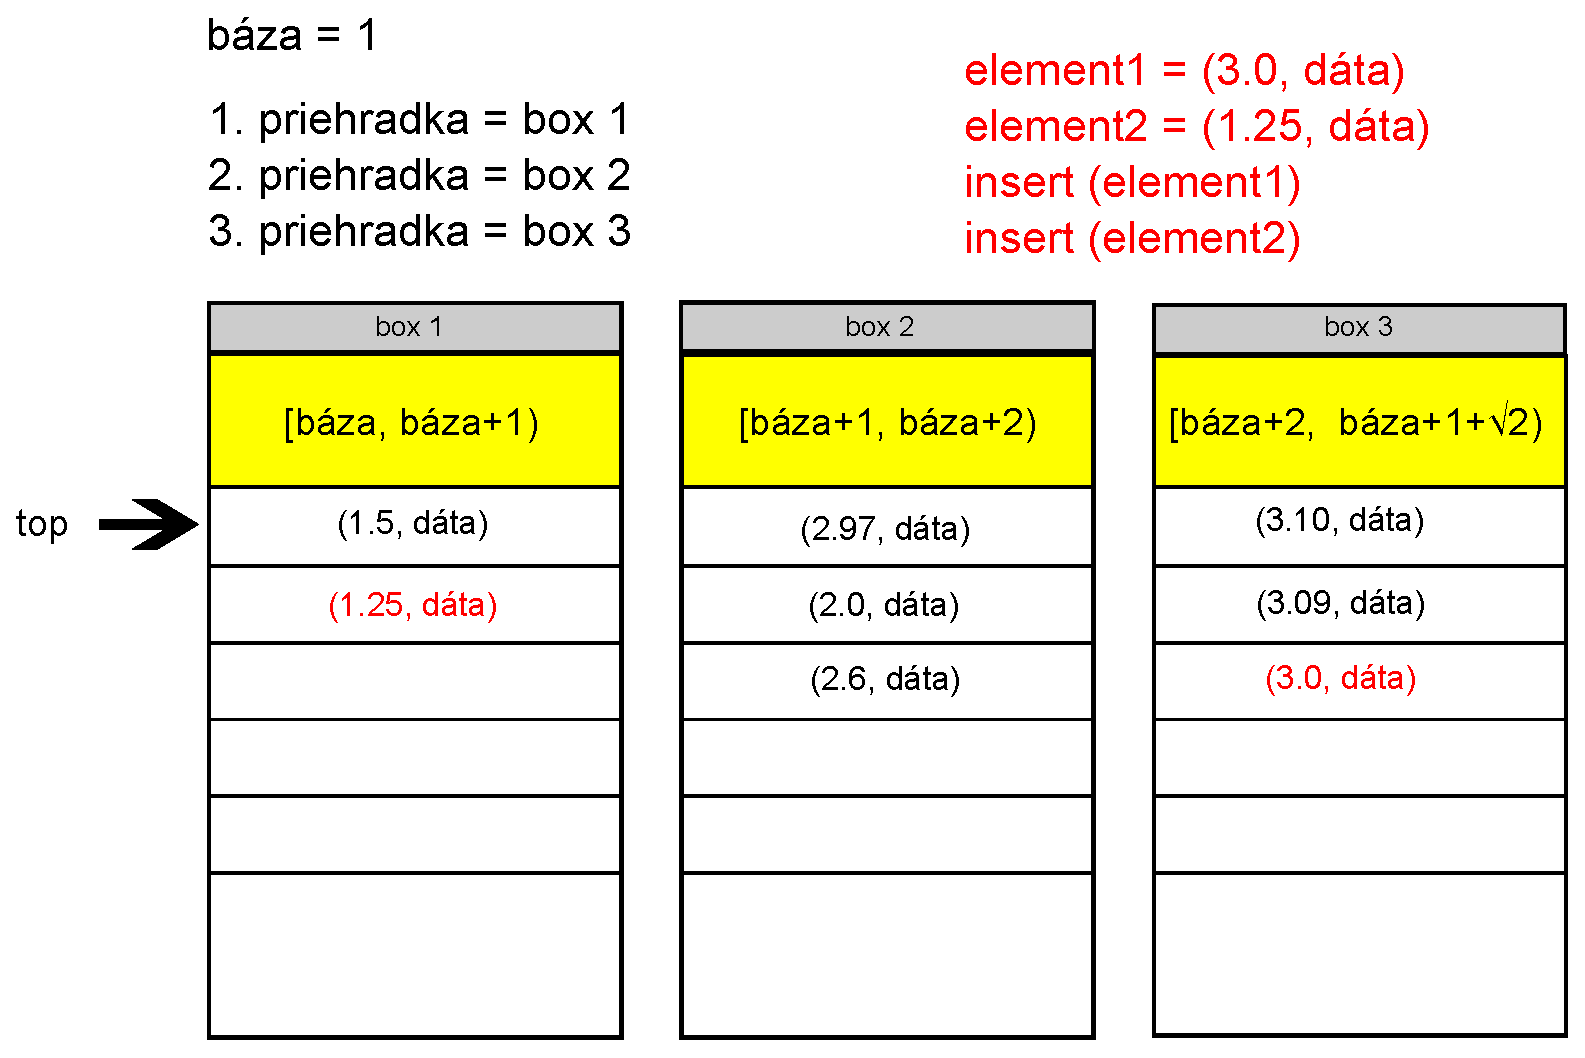
\includegraphics[width=\textwidth]{./img/priehradky_naplnene_default_i.eps}
\caption{Priehradková štruktúra po vložení dvoch vrcholov so vzdialenosťami 1.25 a 3.0. Prvky sa vkladajú stále na koniec priehradok.}
\label{fig:priehradky_i}
\end{figure}


Zmazanie prvku vidíme na obrázku \ref{fig:priehradky_i_d1}.
Celé zmazanie spočíva v inkrementácii ukazovateľa na vrch priehradky.

\begin{figure}[h]
\centering
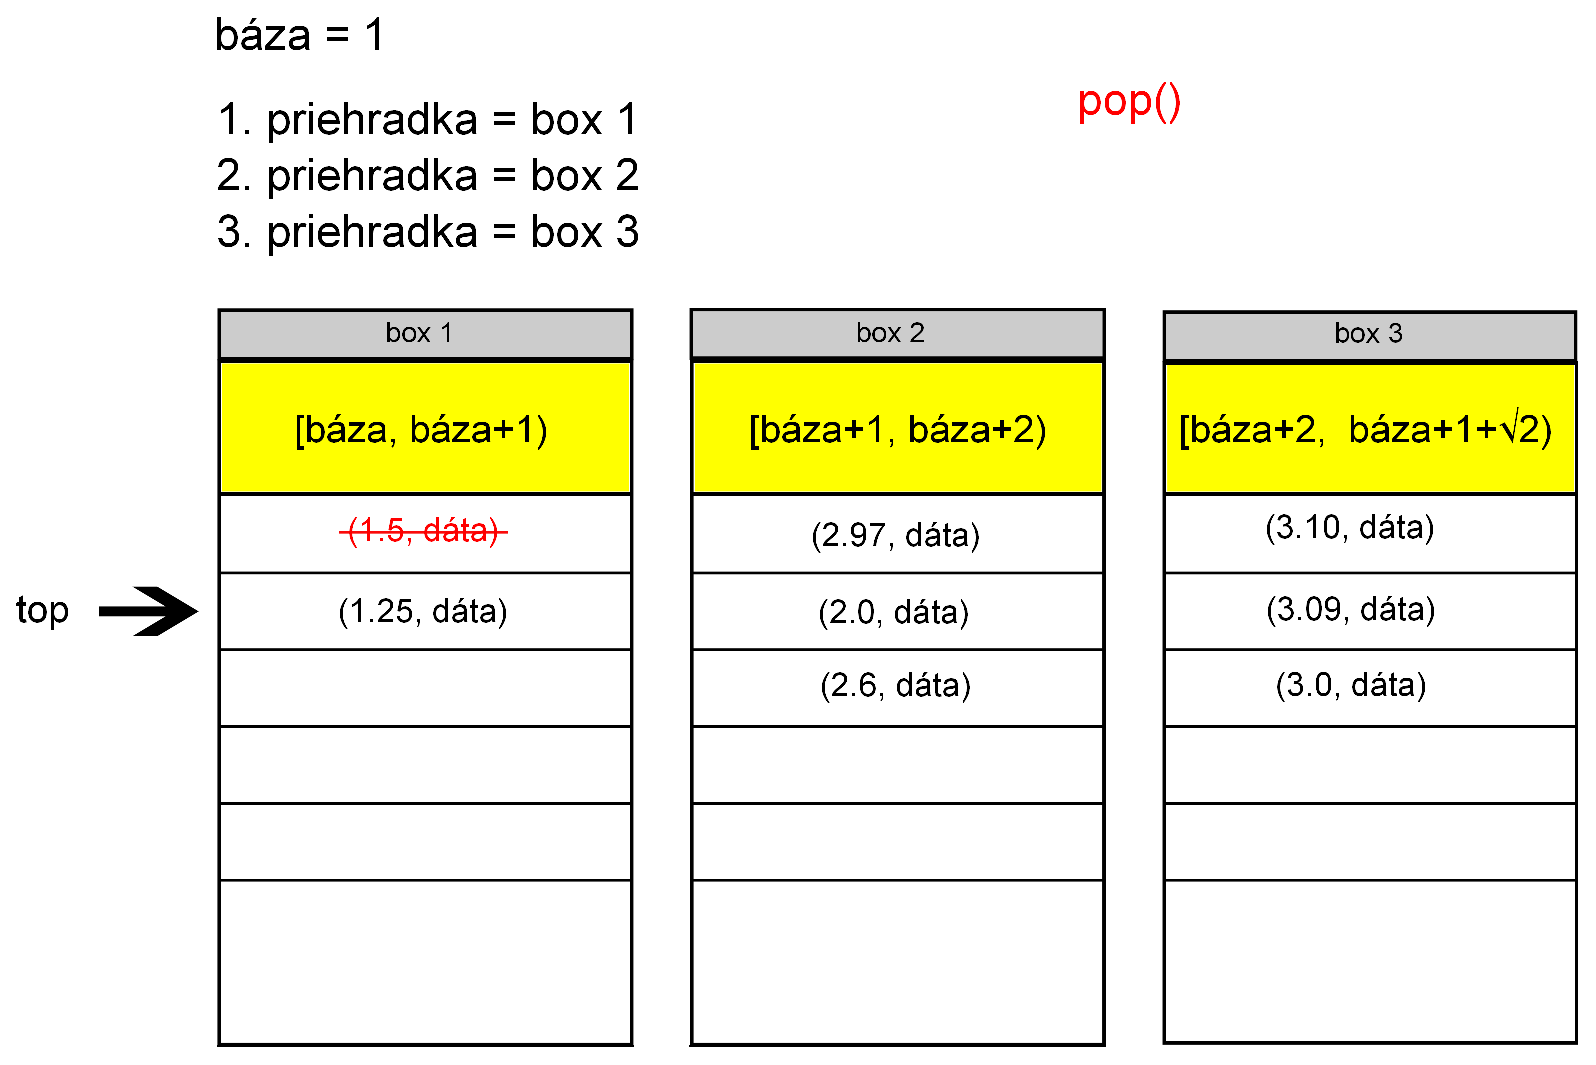
\includegraphics[width=\textwidth]{./img/priehradky_naplnene_default_i_d1.eps}
\caption{Vybranie prvku --- prvok na ktorý ukazuje smerník v prvej priehradke a inkrementujeme ho.}
\label{fig:priehradky_i_d1}
\end{figure}


Pokiaľ sa v priehradke nachádza jediný prvok a ten chceme vybrať, tak nám inkrementácia premennej $ top $ v priehradke 
nepostačí. Musíme prehodiť priehradky. Druhú priehradku presunúť
na miesto prvej, tretiu na miesto druhej a prvú umiestniť nakoniec. Viď obrázok \ref{fig:priehradky_i_d2}. Nakoniec musíme zvýšit bázickú vzdialenosť. Zmena poradia týchto priehradok sa samozrejme uskutočňuje cez prehodenie smerníkov.
Keďže máme konštatný počet priehradok, tak aj táto operácia
trvá konštantný čas.

\begin{figure}[H]
\centering
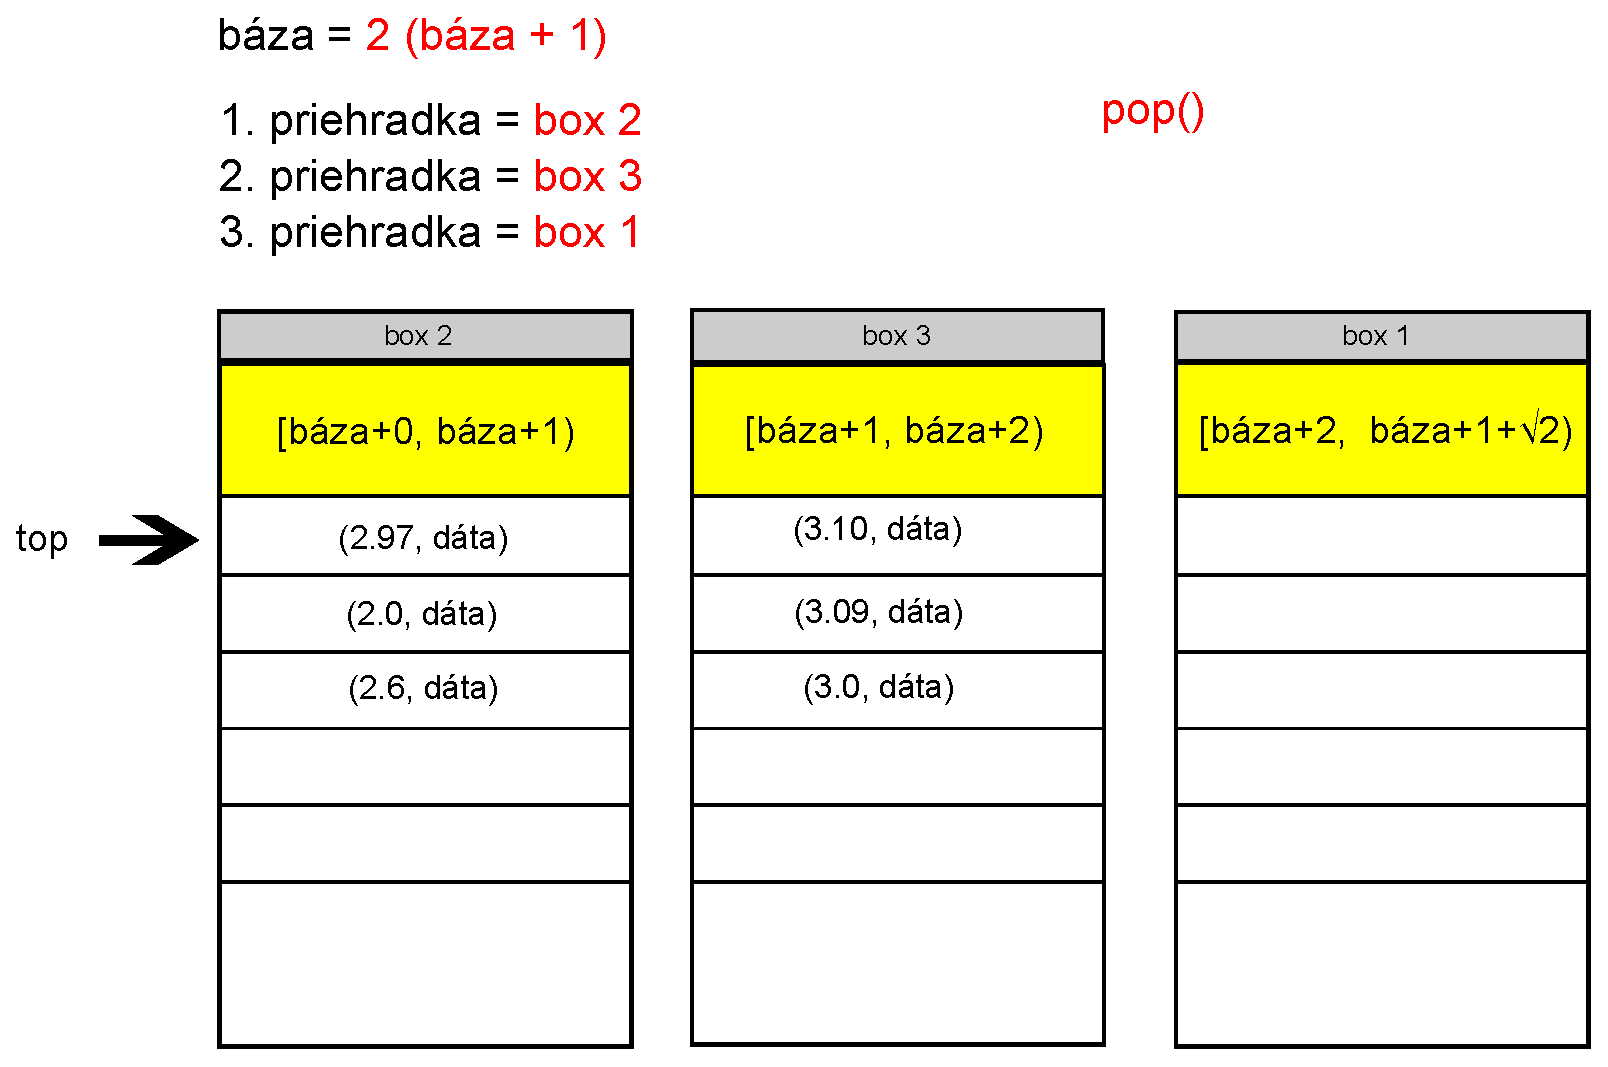
\includegraphics[width=\textwidth]{./img/priehradky_naplnene_default_i_d2.eps}
\caption{Zmazanie posledného prvku prvej priehradky vedie k zmene poradia priehradok}
\label{fig:priehradky_i_d2}
\end{figure}


\begin{theorem}[korektnosť priehradkovej štruktúry]
Dijkstrov algoritmus používajúci haldu $BucketHeap$ vráti korektné najkratšie vzdialenosti do vrcholov grafu.
\end{theorem}
\begin{proof}
Rozsah každej priehradky je ostro menší ako 1. To znamená, že podľa vety~\ref{dinic-observation} a príkladu \ref{ex:range} operácia $pop()$ vracia prvky v poradí, ktoré
nepokazí chod algoritmu. 

Treba ešte dokázať, že tri priehradky postačujú. To je zrejmé,
pretože keď vyberieme vrchol z prvej priehradky, tak jeho vzdialenosť je v rozsahu $[b, b+1)$. Keď prechádzame jeho susedné vrcholy, tak najdlhšia hrana je $ \sqrt{2} $ a teda vzdialenosť k najvzdialenejšiemu susednému vrcholu je ostro menšia, ako $b+1+\sqrt{2}$, čo sa zmestí do intervalu poslednej priehradky.
\end{proof}


\section{A*}
Ďalší algoritmus, ktorým sa budeme zaoberať je algoritmus
A* \cite{astar72} prvykrát popísaný v roku 1968.

Tento algoritmus vychádza z Dijkstrovho algoritmu a je mu veľmi podobný. Hlavný rozdiel medzi týmito algoritmami je, že
kým Dijkstrov algoritmus vyberá z haldy vrcholy s neklesajúcou vzdialenosťou $ d(v) $ od počiatku, tak algoritmus A* vyberá prvky s neklesajúcou vzdialenosťou $ f(v) := d(s,v) + h(v,t) $, kde $ h(v, t) $ značí heuristickú funkciu, ktorá je dolným odhadom vzdialenosti od vrcholu $ v $ do cieľa $ t $. Obrátene, Dijkstrov algoritmus si vieme predstaviť ako algoritmus A*, kde $ \forall v \in G: h(v, t) = 0 $.

Použitá heuristická funkcia má dopad na počet prehľadaných vrcholov a teda do zásadnej miery ovplyvňuje výkon algoritmu.

\subsection{Heuristická funkcia}
 Heuristická funkcia nemôže byť ľubovoľná. Funkcia musí predstavovať tzv. {\sl prípustný potenciál}. Podrobnejší popis sa nachádza napr. na \cite{mares07} \cite{golberg01} \cite{goldbergharrelson05}. Ďalej sa budeme venovať len funkciám, ktoré túto podmienku splňujú.


Najčastejšie heuristické funkcie sú tieto:

\begin{itemize}
\item Euklidovská vzdialenosť.
\item Trojuholníková nerovnosť, tzv. $ landmarks $.
\end{itemize}


\paragraph{Euklidovská vzdialenosť}

Euklidovská vzdialenosť je najjednoduchšie implementovateľná heuristická funkcia. Na väčšine jednoduchých grafov s malým počtom prekážok vracia dobré výsledky. Problém nastáva na grafoch, kde začiatok a koniec cesty sú geometricky blízko seba, hoci ich skutočná vzdialenosť je veľká.
Príklad vidíme na obrázku \ref{fig:antieuclid}.
TODO?? pozor na blbe rozdelenie obdlznikov - ja to ratam 
aj cez sikme hrany atd atd


\begin{figure}[H]
\centering
\includegraphics[width=0.5\textwidth]{./img/antieuclid505d.jpg}
\caption{Mapa, na ktorej euklidovská heuristika zlyhá.}
\label{fig:antieuclid}
\end{figure}


\paragraph{Landmarks a trojuholníková nerovnosť}
Nevýhoda použitia euklidovskej heuristickej funkcie je na obecných mapách zjavná. To motivovalo vymyslieť heuristiku, ktorá lepšie odráža vzdialenosti v grafe.

Jednou z týchto heuristík je počítanie dolného odhadu pomocou tzv. {\sl landmarks}. 

Landmarks sú vybrané vrcholy v grafe, z ktorých je následne prepočítaná najkratšia vzdialenosť do všetkych ostatných
vrcholov grafu. 



Kedže jeden prechod grafu vieme Dijkstrovým algoritmom s priehradkami vykonať za lineárny čas, predpočítanie $ k $ landmarkov trvá $ \BigO{kn} $, kde $n$ značí počet vrcholov grafu.


TODO?? ako to funguje...

\subparagraph{Možnosti voľby landmarkov}

Pri voľbe landmarkov sú dva faktory: počet a rozmiestnenie.

\begin{example}[na počte záleží]
Pokiaľ zvolíme málo landmarkov, tak dolný odhad nebude presný.
Pokiaľ ich zvolíme priveľa, tak prepočet vzdialenosti cez každý landmark pre každý vrchol zaberie veľa času.
\end{example}

\begin{example}[na rozmiestnení záleží]
Pokiaľ zvolíme všetky landmarky hneď pri sebe, tak heuristika
nám nebude vraciať dostatočne presné dolné odhady na vzdialenosť vrcholov, ktoré sú ďaleko od landmarkov.
\end{example}


TODO??potencialy euklid landmarks landmark selection priblem s priehradkami
\part{Implementácia}
\chapter{Súťažný algoritmus}
Súťažný algoritmus bude využívať poznatky popísané v predošlej kapitole. Navyše zavedieme koncept tzv. {\sl mriežkového grafu bez prekážok}, ktorý umožní mierne zrýchliť výkon algoritmu v mnohých prípadoch, väčšinou však pri trasách, kde počiatočný a koncový bod ležia relatívne \uv{blízko seba}.


\section{Mriežkový graf bez prekážok}
Nie všetky najkratšie cesty musia obchádzať veľa prekážok. 
V mnohých prípadoch neleží medzi počiatočným a koncovým bodom žiadna prekážka, a~teda cesty sú veľmi priamočiare. To sa pokúsime využiť na~zlepšenie výkonu algoritmu.
Pre ľahšie vyjadrovanie si zaveďme definíciu {\sl mriežkového grafu bez prekážok}.

\begin{define}
{\sl Mriežkový graf je bez prekážok}, 
pokiaľ medzi každými dvoma susednými vrcholmi existuje hrana.
\end{define}
Kvôli lepšej prehľadnosti a stručnosti budeme mriežkový graf bez prekážok nazývať aj {\sl obdĺžnik}.
Intuitívne, kvôli jeho vizuálnej predstave. Jeho obsahom bude počet vrcholov patriacich do tohto obdĺžniku.

Majme mriežkový graf bez~prekážok a~hľadajme najkratšiu cestu medzi bodmi $s=(x_s,y_s), t=(x_t,y_t)$.
V~tomto prípade vieme nájsť najkratšiu cestu veľmi jednoducho.

\begin{algorithm}
\caption{Nájdi najkratšiu cestu medzi dvoma bodmi $s$ a $t$ na mriežkovom grafe bez prekážok}
\label{alg1}
\begin{algorithmic}[1] % number one = line numbering is on
\REQUIRE $s=(x_s,y_s), t=(x_t,y_t)$
\ENSURE $path$


\STATE path.append($(x_s, y_s)$)
\COMMENT {pridám počiatok}

\WHILE {$x_s \neq x_t \vee y_s \neq y_t $}
	\IF {$x_s < x_t$}
		\STATE $x_s \leftarrow x_s + 1$
	\ELSIF {$x_s > x_t$}
		\STATE $x_s \leftarrow x_s - 1$
	\ENDIF

	\IF {$y_s < y_t$}
		\STATE $y_s \leftarrow y_s + 1$
	\ELSIF {$y_s>y_t$}
		\STATE $y_s \leftarrow y_s - 1$
	\ENDIF
	\STATE path.append($(x_s, y_s)$)
\ENDWHILE

\end{algorithmic}
\end{algorithm}



Jednoducho povedané: keď sa počiatočný a koncový bod líšia v jednej súradnici, tak sa posúvame priamočiaro,
keď sa líšia v oboch, tak sa posúvame šikmo.


Pokiaľ si zadefinujeme 
$ dx := |x_t - x_s|$ 
a
$ dy :=|y_t - y_s| $
 , tak počet vrcholov,
ktorými cesta prechádza vieme zhora odhadnúť, ako $\max(dx, dy)$. Jej vzdialenosť vieme zistiť v čase  $\BigO{\max(dx, dy)}$
Na zistenie vzdialenosti v každom kroku nám postačí konštantná pamäť.


Pokiaľ sa počiatočný a koncový bod cesty nachádza v jednom obdĺžniku, tak vieme pomocou tohto algoritmu veľmi rýchlo nájsť najkratšiu cestu.
Jediným problémom ostalo rozdeliť mriežkový graf na tieto obdĺžniky. 


\section{Hľadáme obdĺžniky}
Našou snahou je dekomponovať mriežkový graf do obdĺžnikov tak, aby bola čo najväčšia pravdepodobnosť toho, že 
dva náhodne zvolené body (začiatok a koniec) ležia v jednom obdĺžniku. Čiže aby sa dalo toto zrýchlené
hľadanie najkratšej cesty použiť v najväčšom možnom počte prípadov.


\subsection{Proporcie obdĺžnikov}

Dôležitou otázkou je, na akých vlastnostiach obdĺžnikov záleží. Uvažujme nasledujúci motivačný príklad.
\begin{example}
Majme na mriežkovom grafe nájdené dva obdĺžniky, ktoré dovedna pokrývajú 10 vrcholov.
Predstavme si tieto dva prípady. V prvom prípade prvý pokrýva 9 vrcholov, druhý 1. V druhom prípade obdĺžniky pokrývajú 6 vrcholov a 4 vrcholy.
Chceme maximalizovať pravdepodobnosť toho, aby pri voľbe dvoch náhodných bodov boli oba body v rovnakom obdĺžniku.
\end{example}

Úlohu vieme zobecniť na klasickú pravdepodobnostno-optimalizačnú úlohu.

\begin{example}
Máme $k$ ekvivalenčných tried na množine s $n$ prvkami. Ako zvoliť ekvivalenčné triedy tak, 
aby pri voľbe dvoch náhodných prvkov bola pravdepodobnosť toho, 
že oba prvky budú v tej istej ekvivalenčnej triede čo najvyššia?
\end{example}

\begin{note}
Ekvivalenčnú triedu predstavuje obdĺžnik a množinu predstavuje množina vrcholov grafu.
Alternatívne sa môžeme na úlohu pozerať ako na problém farbenia $n$ guličiek pomocou $k$ farieb.
\end{note}

Zapíšme túto úlohu formálne. Majme $n$-prvkovú množinu $Prv = \{x_1,\ldots,x_n\}$, $k$-prvkovú množinu ekvivalenčných tried $Ek = \{ek_1,\ldots, ek_k\}$, veľkosť 
triedy $\|ek_i\|$ označme $k_i$ a zaveďme funkciu $f \colon Prv \to Ek$ ktorá roztriedi prvky do ekvivalenčných tried.

Označme výberový priestor $\Omega = \{(x_a, x_b) | x_a, x_b \in Prv, a \not= b \}$.
Udalosťou $A_i$ nazveme jav, v~ktorom oba prvky patria do tej istej ekvivalenčnej triedy $ek_i$,
teda $A_i = \{(x_a, x_b) | x_a, x_b \in Prv, a \not= b, f(x_a) = f(x_b) = ek_i \}$.
Jav $A = \bigcup_{i=1}^{k} A_i$ teda nastáva práve vtedy,
 keď oba vybrané prvky patria do rovnakej triedy.

Úlohou je navrhnúť funkciu $f$ tak, aby pravdepodobnosť $P[A]$ bola čo najvyššia. 
Keďže udalosti $A_i$ sú nezlučiteľné, môžme písať 
$P[A] = P[\bigcup_{i \in Ek} A_i] = \sum_{i \in Ek}P[A_i]$.

Ak si pravdepodobnosť každého javu rozpíšeme, dostaneme 
$\sum_{i \in Ek}P[A_i] = \sum_{i = 1}^{k} \frac{{{k_i} \choose {2}}}{{{|Prv|} \choose {2}}}$.


Keďže chceme nejak rozvrhnúť prvky v triedach $ek_i$, a menovateľ je konštanta, môžme ho vynechať.

Maximalizujeme hodnotu výrazu 
$\sum_{i = 1}^{k} {{k_i} \choose {2}} = \sum_{i = 1}^{k} {\frac{k_i!}{(k_i -2 )!2!}} = \sum_{i = 1}^{k}{\frac{k_i (k_i-1)}{2}}$.
Po vyškrtnutí konštanty a roznásobení sme dostali nasledujúcu optimalizačnú úlohu:
maximalizovať $\sum_{i = 1}^{k} {k_i^2 - k_i}$ za podmienok $\sum_{k=1}^{k}k_i = n$,
kde $k_i \in \N_0$.

Sumu si vieme rozpísať ako 
$\sum_{i = 1}^{k} {k_i^2 - k_i} = \sum_{i = 1}^{k} {k_i^2} + \sum_{i = 1}^{k}{-k_i}$
druhá suma sa nasčíta na $-n$, čo je konštanta, takže nám stačí maximalizovať 
$\sum_{i = 1}^{k} {k_i^2}$.

Teraz nám už len zostáva použiť nerovnosť
$(a+b)^2 \geq a^2 + b^2$, ktorá platí pre $a,b \geq 0$, z ktorej jasne vyplýva, že potrebujeme spraviť ľubovoľné $k_i$ čo najväčšie
a teda aj ekvivalenčné triedy musia byť čo najväčšie.

Potrebujeme teda nájsť obdĺžniky s~najväčším možným obsahom. 
V~programe tento problém rieši trieda Colorizator.
Tá v grafe nájde najväčší obdĺžnik a \uv{ofarbí} ho jednou farbou.
Na zvyšnom neofarbenom grafe znovu hľadá najväčší obdĺžnik a ofarbí ho inou farbou, atď.
Farbenie skončí, keď obsah najväčsieho obdĺžnika je menší ako 500.


\subsection{Nájdenie najväčšej jednotkovej podmatice}
Ako sme si v~úvode povedali, mriežkovú mapu vieme reprezentovať ako maticu, čiže
problém môžeme ekvivalentne zapísať ako problém hľadania najväčšej jednotkovej podmatice.
Tento problém má riešenie v~čase lineárnom od~počtu vrcholov, takže nájdenie $k$ najväčších
jednotkových matíc trvá $\BigO{k \cdot n}$, kde $n$ je počet vrcholov matice.

Slovný popis algoritmu \ref{alg:largest_submatrix}: 
V~prvom prechode maticou si u~každého vrcholu zapamätáme počet jedničiek naľavo od neho, vrátane daného vrcholu. 
Tento prechod trvá lineárny čas.

V~druhom prechode algoritmus prejde zaradom všetky stĺpce zľava doprava.
Každý stĺpec prechádzame odhora nadol a zisťujeme, aký je najväčší obsah obdĺžnika, ktorého horný pravý roh je práve prechádzaný prvok.
Pričom vy TODO??


\begin{algorithm}
\caption{Nájdenie najväčšej jednotkovej podmatice v matici  $m$x$n$}
\label{alg:largest_submatrix}
\begin{algorithmic}[1] % number one = line numbering is on
\REQUIRE matica $M$ rozmerov $m \times n$ nad telesom $\Z_2$
\ENSURE pravý dolný roh podmatice aj s jej rozmermi


\FORALL {prvok $p$, $p \in M$}
	\IF {$p = 0$}
		\STATE nalavoOdPrvku(p) $\leftarrow$ 0
	\ELSE
		\STATE nalavoOdPrvku(p) $\leftarrow$ najdlhšia súvislá postupnosť jednotiek končiaca prvkom $p$
	\ENDIF	
\ENDFOR

\FOR {stĺpec $s$, $s \in M$ }
	\STATE Vytvor nový zásobník dvojice čísel (riadok, nalavoOdPrvku)
	\FOR {riadok $r$, $r \in M$ }
		\STATE $p \leftarrow (s, r)$
		
		\WHILE {Zásobník je neprázdny}
			\STATE vyberiem prvok $top$ z vrcholu zásobníka
			\IF {$top$.nalavoOdPrvku $>$ nalavoOdPrvku(p)}
						
				\STATE prvokZoZasobnika $\leftarrow$ ($top$.r, s)
				\STATE DlzkaSekvencie(prvokZoZasobnika) = r - prvokZoZasobnika.r
			
			\ELSE
				\STATE Vložím prvok $prvokZoZasobnika$ do zásobníka
				\STATE break
			\ENDIF
		\ENDWHILE
		
		\STATE Do zásobníka vložím dvojicu (r, nalavoOdPrvku(p))
	\ENDFOR
	
	\STATE // prešli sme stĺpec, teda skončíme
	\WHILE {Zásobník je neprázdny}
		\STATE vyberiem prvok $top$ z vrcholu zásobníka
		\STATE prvokZoZasobnika $\leftarrow$ ($top$.r, s)
		\STATE DlzkaSekvencie(prvokZoZasobnika) = m - prvokZoZasobnika.r
		
	\ENDWHILE
\ENDFOR




\end{algorithmic}
\end{algorithm}



TODO: pridaj obrazok mapy a jej dekompozicie opdla farieb
\chapter{Testovanie a výsledky}

\section{Kritériá a popis testovania}
\subsection{Vstupné dáta}
Častým problémom pri vzájomnom porovnávaní algoritmov je
nájsť testovaciu vzorku, ktorá by otestovala beh algoritmu na širokej škále grafov.
Ako bolo v úvode spomenuté, súťaž {\sl Grid-Based Path Planning Competition} poskytuje množstvo máp rôznych typov a rozmerov,
na ktorých sa algoritmy dajú testovať. Formát máp popisuje článok \cite{sturtevant2012benchmarks}.

Programy boli testované na troch mapách. Ich grafická reprezentácia bola 
vytvorená pomocou programu T-map (popis programu a významu farieb sa nachádza v prílohe \ref{userdoc}) 
a~môžme ju vidieť na obrázkoch Obr.~\ref{fig:aftershock_map},~Obr.~\ref{fig:brushfire_map} a Obr.~\ref{fig:biggamehunters_map}.
Pripomeňme si, že žltou farbou je označená priechodná oblasť; ostatné oblasti sú nepriechodné.

Každá mapa bola testovaná oproti dvom množinám vstupov.
Každá z týchto množín obsahuje približne 200 dopytov
 na~najkratšiu vzdialenosť medzi dvojicou zadaných bodov.
Jedna z tých dvoch množín obsahuje dvojice bodov, ktoré ležia relatívne \uv{blízko} seba, druhá množina obsahuje dvojice bodov, medzi ktorými je vzdialenosť väčšia.


Konkrétne máme tieto 4 vstupné súbory:
\begin{itemize}
\item AS --- vstupný súbor k mape Aftershock obsahujúci \uv{blízke} body.
\item AL --- vstupný súbor k mape Aftershock obsahujúci vzdialenejšie body.
\item BS --- vstupný súbor k mape Brushfire obsahujúci \uv{blízke} body.
\item BL --- vstupný súbor k mape Brushfire obsahujúci vzdialenejšie body.
\item GS --- vstupný súbor k mape BigGameHunters obsahujúci \uv{blízke} body.
\item GL --- vstupný súbor k mape BigGameHunters obsahujúci vzdialenejšie body.
\end{itemize}


\begin{figure}[H]
\centering
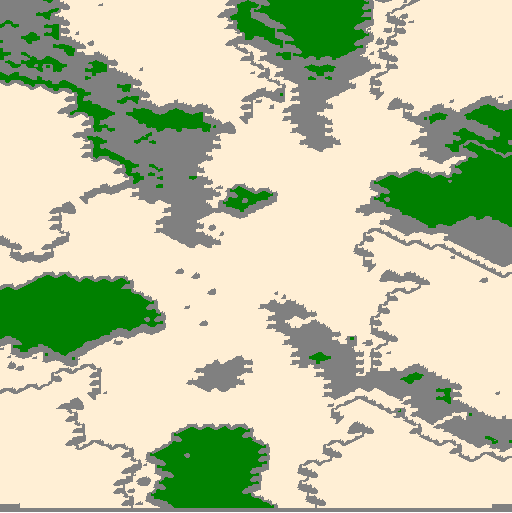
\includegraphics[width=10cm]{./img/Aftershock.png}
\caption{Graf \uv{Aftershock}}
\label{fig:aftershock_map}
\end{figure}

\begin{figure}[H]
\centering
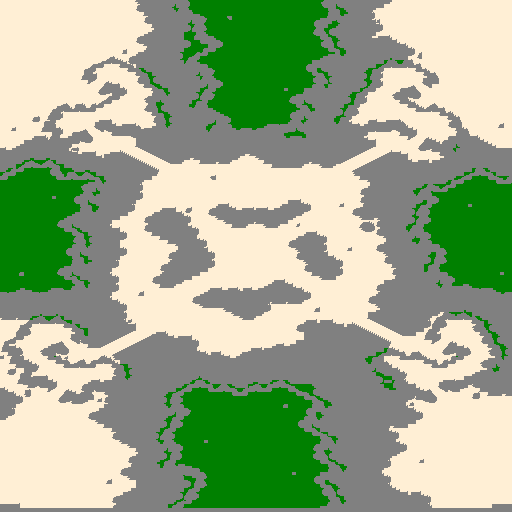
\includegraphics[width=10cm]{./img/Brushfire.png}
\caption{Graf \uv{Brushfire}}
\label{fig:brushfire_map}
\end{figure}

\begin{figure}[h]
\centering
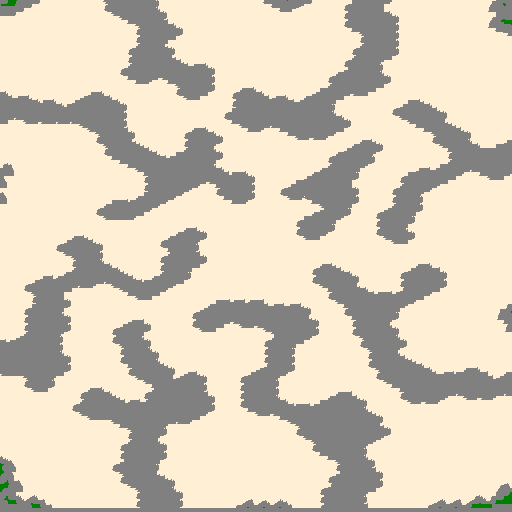
\includegraphics[width=10cm]{./img/BigGameHunters.png}
\caption{Graf \uv{BigGameHunters}}
\label{fig:biggamehunters_map}
\end{figure}

\subsection{Testovacie kritériá}
Algoritmy testujeme podľa nasledovných kritérií:

\begin{itemize}
\item Rýchlosť nájdenia cesty.
\item Dĺžka trasy.
\item Počet prehľadaných vrcholov.
\end{itemize}


\subsection{Testované algoritmy}
Testovať budeme nasledujúce algoritmy:
\begin{itemize}
\item Dijkstrov algoritmus nad binárnou haldou (označíme DH).
\item Dijkstrov algoritmus nad priehradkovou haldou (označime DBQ).
\item A* používajúci 6 landmarkov (označíme A*).
\item A* používajúci 6 landmarkov a taktiež obdĺžnikovú dekompozíciu, popísanú v kapitole 3 (označíme A*+).
\item Anderson -- s prehľadom najrýchlejší algoritmus, ktorý vyhral súťaž (označíme And).
\end{itemize}


\subsection{Kompilácia}
Kód bude kompilovaný kompilátorom g++ s direktívou \emph{-O3}, čo zaručuje maximálnu rýchlosť a efektivitu behu programu.


\section{Výsledky}

\begin{table}[H]
	\centering
	\begin{tabular}{|l | r|r|r|r|r|r|}
	\hline
	  & AS & AL & BS & BL & GS & GL \\
	\hline
	DH & 8.706919 & 8.609133 & 4.554813 & 3.803920 & 11.059045 & 7.932771 \\
	DBQ & 0.506893 & 11.505914 &  0.329444 & 4.315670 & 0.467251 & 11.990992 \\
	A* & 0.263951 & 7.481771 & 0.283890 & 15.599357 & 0.393476 & 9.667814 \\
	A*+  & 0.182731 & 7.502437 &  0.197504 & 15.670339 & 0.257229 & 9.694499\\
	And  &  0.000543 & 0.002659 & 0.000359 & 0.001747 & 0.000673& 0.002197\\
	\hline
	\end{tabular}
	\caption{Výsledky časov v sekundách}
	\label{fig:totaltime_result}
\end{table}


\begin{table}[H]
	\centering
	
	\begin{tabular}{|l | r|r|r|r|r|r|}
		\hline
		  & AS & AL & BS & BL & GS & GL \\
		\hline
		DH & 20888032 & 26585115 & 14967159 & 15403707 & 25967574 & 22755932 \\
		DBQ & 1347329 & 39028967 & 1176089 & 20528587 & 1255147 & 40707226 \\
		A* & 350839 & 13854096& 624561 & 41883515 & 637189 & 17936238 \\
		A*+ & 250022& 13854096 & 465311 & 41883515 & 407731 & 17936238 \\

		\hline
	\end{tabular}
		
	\caption{Výsledky obsahujúce počet navštívených vrcholov}
	\label{fig:verticesscanned_result}
\end{table}

\begin{table}[H]
	\centering
	\begin{tabular}{|l | r|r|r|r|r|r|}
	\hline
	 & AS & AL & BS & BL & GS & GL \\
	\hline
	DH & 111010 & 548861 & 78330.7& 326556 & 82873.9 & 395860 \\
	DBQ & 8710.17 & 548861 & 8731.65 & 152185 & 8744.62 & 128398 \\
	A* & 8743.7 & 144527& 8762.74 & 153288 & 8774.98 & 128885 \\
	A*+ & 8738.43& 144527 & 8758.98 & 153288 & 8769.46 & 128885 \\
	And & 22057.2 & 144854 & 22010 & 156927 & 27717.8 & 135411 \\
	\hline
	\end{tabular}
	\caption{Výsledky obsahujúce prejdeny vzialenosť}
	\label{fig:totalpath_result}
\end{table}


\include{tmaps}
% Ukázka použití některých konstrukcí LateXu (odkomentujte, chcete-li)
%\include{ukazka}

\chapter*{Záver}
\addcontentsline{toc}{chapter}{Záver}

Práca sa zaoberala hľadaním ciest na mriežkových grafoch s dôrazom na rýchlosť nájdenia cesty a dĺžku nájdenej cesty. 


%%% Seznam použité literatury
%%% Seznam použité literatury je zpracován podle platných standardů. Povinnou citační
%%% normou pro bakalářskou práci je ISO 690. Jména časopisů lze uvádět zkráceně, ale jen
%%% v kodifikované podobě. Všechny použité zdroje a prameny musí být řádně citovány.

\def\bibname{Zoznam použitej literatúry}
\begin{thebibliography}{99}
\addcontentsline{toc}{chapter}{\bibname}
%%%%

\bibitem{euler41}
	L. Euler. 
	\emph{Solutio problematis ad geometriam situs pertinentis}.
    Commentarii academiae scientiarum Petropolitanae, 8:128–140, 1741.

\bibitem{dijkstra59}
  E. W. Dijkstra.
  \emph{A note on two problems in connexion with graphs}.
  Numerische Mathematik, 1(1):269--271, 1959.

\bibitem{floyd62}
R.~W. Floyd.
\newblock Algorithm 97: Shortest path.
\newblock {\em Commun. ACM}, 5(6):345--, June 1962.



\bibitem{mares07}
  M. Mareš.
  \emph{Krajinou grafových algoritmů}.
  ITI Series, Prague 2007 [ONLINE]. [CIT. 2013-7-21]. Dostupné z \url{http:
  //mj.ucw.cz/vyuka/ga/}.
  
\bibitem{astar72}
P.~E. Hart, N.~J. Nilsson, B. Raphael.
\newblock Correction to a formal basis for the heuristic determination of minimum cost paths.
\newblock {\em SIGART Bull.}, (37):28--29, December 1972.

\bibitem{golberg01}
A. V. Goldberg. 
\emph{Shortest Path Algorithms: Engineering Aspects}. 
In Proc. ESAAC '01, Lecture Notes in
Computer Science. Springer-Verlag, 2001.


\bibitem{goldbergharrelson05}
A. V. Goldberg, C. Harrelson. 
\emph{Computing the Shortest Path: A* Search Meets Graph Theory}.
In Proc. 16th ACM-SIAM Symposium on Discrete Algorithms, pages 156--165, 2005.

\bibitem{asymptotic65}
 J. Hartmanis, R. Stearns. 
 \emph{On the computational complexity of algorithms}. 
 Transactions of the American Mathematical Society, vol. 117, 285--306, 1965.

\bibitem{sturtevantgppc}
  N.~Sturtevant.
  \emph{GPPC: Grid-Based Path Planning Competition} [ONLINE] 2013. [CIT. 2013-7-21].
  Dostupné z: \url{http://movingai.com/GPPC/}. 
   
\bibitem{sturtevant2012benchmarks}
N.~Sturtevant.
\newblock Benchmarks for grid-based pathfinding.
\newblock {\em Transactions on Computational Intelligence and AI in Games},
  4(2):144 -- 148, 2012.
   
\bibitem{gs97}
A.~Goldberg, C. Silverstein.
\emph{Implementations of Dijkstra’s Algorithm Based on Multi-Level Buckets}.
Springer Berlin Heidelberg,
1997.

\bibitem{krasner_mvc_1988}
G.~Krasner, S.~Pope.
\newblock A description of the {Model-View-Controller} user interface paradigm
  in the smalltalk-80 system.
\newblock {\em Journal of Object Oriented Programming}, 1(3):26--49, 1988.

\bibitem{agrawal_largest_submatrix}
A. Agrawal.
\emph{Find largest sub-matrix with all 1s (not necessarily square)} [ONLINE] 2011. [CIT. 2013-7-21]. Dostupné z
\url{http://tech-queries.blogspot.cz/2011/09/find-largest-sub-matrix-with-all-1s-not.html}





\end{thebibliography}


%%% Tabulky v bakalářské práci, existují-li.
\chapwithtoc{Zoznam tabuliek}

%%% Použité zkratky v bakalářské práci, existují-li, včetně jejich vysvětlení.
\chapwithtoc{Zoznam použitých skratiek}

%%% Přílohy k bakalářské práci, existují-li (různé dodatky jako výpisy programů,
%%% diagramy apod.). Každá příloha musí být alespoň jednou odkazována z vlastního
%%% textu práce. Přílohy se číslují.
\chapwithtoc{Prílohy}

\openright
\end{document}
